\chapter{Theoretical Background}
Since Turing wrote about the imitation game\cite{imitationgame} and Rosenblatt about the perceptron\cite{perceptron}, learning machines have stayed in the minds of computer scientists and science fiction writers. 
Improvements in computation and algorithms have since then taken machine learning(ML) past human level performance in multiple areas such as image recognition\cite{youtubecats}\cite{deepface}, board games like chess\cite{alphazero} or go\cite{alphago}, TV game-shows like Jeopardy\cite{jeopardy} or e-sports such as DOTA2\cite{dota2}.

\section{Machine Learning}
\label{background:ML}
 
In machine learning, the fields of statistics, mathematics and data analysis are combined and applied to automatic modeling of data. Its three main sub-fields, supervised, unsupervised and reinforcement learning covers a vast number of structures and techniques, but in this thesis we will focus on the flag-ship of machine learning, the artificial neural network, and set it in a supervised learning scenario where it is applied to a classification problem.

\begin{figure}[ht] 
\centering
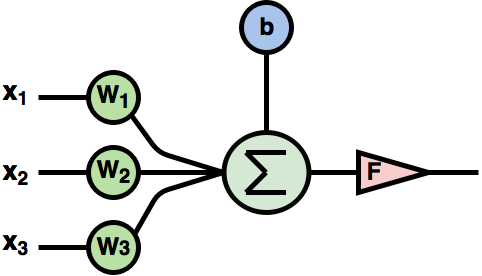
\includegraphics[width=0.7\linewidth]{Chapters/2.Background/figures/artificial_neuron.png}
\caption[Visualization of a artificial neuron]{Visualization of a artificial neuron. Each input \(x_{i}\) is multiplied with a corresponding trainable weight \(W_{i}\) before the products are all summed together with a bias \(b\). The resulting value is then passed through a activation function \(F\)}
\label{fig:artificialneuron}
\end{figure}

Supervised learning is a way to teach some machine learning system patterns in annotated data. In a data set \(\left [X, Y \right] \), each data-point \(x_{i}\) corresponds to a label or ground truth \(y_{i}\). In the context of a Artificial Neural Network, each \(x_{i}\) is fed through the network and fitted against the target \(y_{i}\) using some optimization algorithm. 

Inspired by the structure of the brain, the \textit{Artificial Neural Network} or \textit{Neural Network} (NN) consists of layers of artificial neurons like the one visualized in figure \ref{fig:artificialneuron}. Each neuron has a number \(n\) of inputs \(x_{i}\) where each input is scaled by a tunable parameter or \textit{weight} \(w_{i}\) and summed together including a bias \(b\) before it is passed through a activation function \(F\).

\begin{equation}
    F(\sum_{i=1}^{n}W_{i}x_{i} + b) = output
\end{equation}

Two of the most commonly used activation functions are the rectified linear unit function (ReLU) and the softmax function, which is the generalization of binary logistic regression to multiple classes. ReLU simply evaluates to the maximum of neuron output and 0, which sets zero if the output is negative and keeps positive outputs. Softmax on the other hand approximates a probability by scaling the output of a set of neurons to have a sum between 0 and 1 and are used in classification. These two activation functions will play a role in the later experiments (see \ref{exp1:implementation} and \ref{exp2:implementation}) in this thesis, where softmax will be used as the final activation layer to be the basis of classification. ReLU is used as activation function throughout the rest of the neural networks. 

These types of systems \textit{learn} to approximate a function based on the data provided to the network. Each data point x consist of multiple features (\(x_{i}\)'s), which is fed through one or more layers of neurons that outputs an prediction \(\hat{y}_{i}\). This prediction is then compared to the ground truth with a loss function\footnote{Also called cost function, error function or objective function} which calculates the difference between expected output \(y_{i}\) and observed output \(\hat{y}_{i}\). Here also there is a multitude of functions which will not be discussed. For the purpose of classification in this thesis, the loss function we will use is a cross-entropy function which is well suited for classification with the softmax activation output\cite{softmaxcrossentropy}.

The goal of the training is to minimize the loss function for a given data set. To accomplish this, the loss is backpropagated through the neural network and an optimization algorithm is used to calculate the gradient of the weights with regards to the layer output and then to adjust the weights. The optimizers used in the experiments \ref{exp1} and \ref{exp2} are stochastic gradient descent(SGD)\cite{sgd} and Adaptive Moment Estimation (Adam)\cite{adam}. 

Neural Networks function approximation properties can be used in regression in data analysis or reward signal estimation in reinforcement learning among other things, but are as mentioned applied to classification in this thesis. 
The final softmax layer outputs an estimated probability for each label given some input where the label given highest probability is selected as the models prediction. As long as the input features to the network is correlated to the label in some way and there is enough training data, the neural network will adapt to the patterns in input features and learn one or more classification rules. In the case of a image classification problem, the network is provided with the raw pixel values in the image. A normal, fully connected neural network\footnote{Also called affine or dense networks or layers} is badly suited for this type of classification since attributes in images often change location or scale in the images \ref{exp1:implementation}. E.g: a picture of a dog is still a image of a dog if you rotate the image upside down, zoom in on the dog or frame the image differently. To account for all these cases, the data set used would have to contain enough examples of all these variations.
\begin{figure}[ht] 
    \centering
    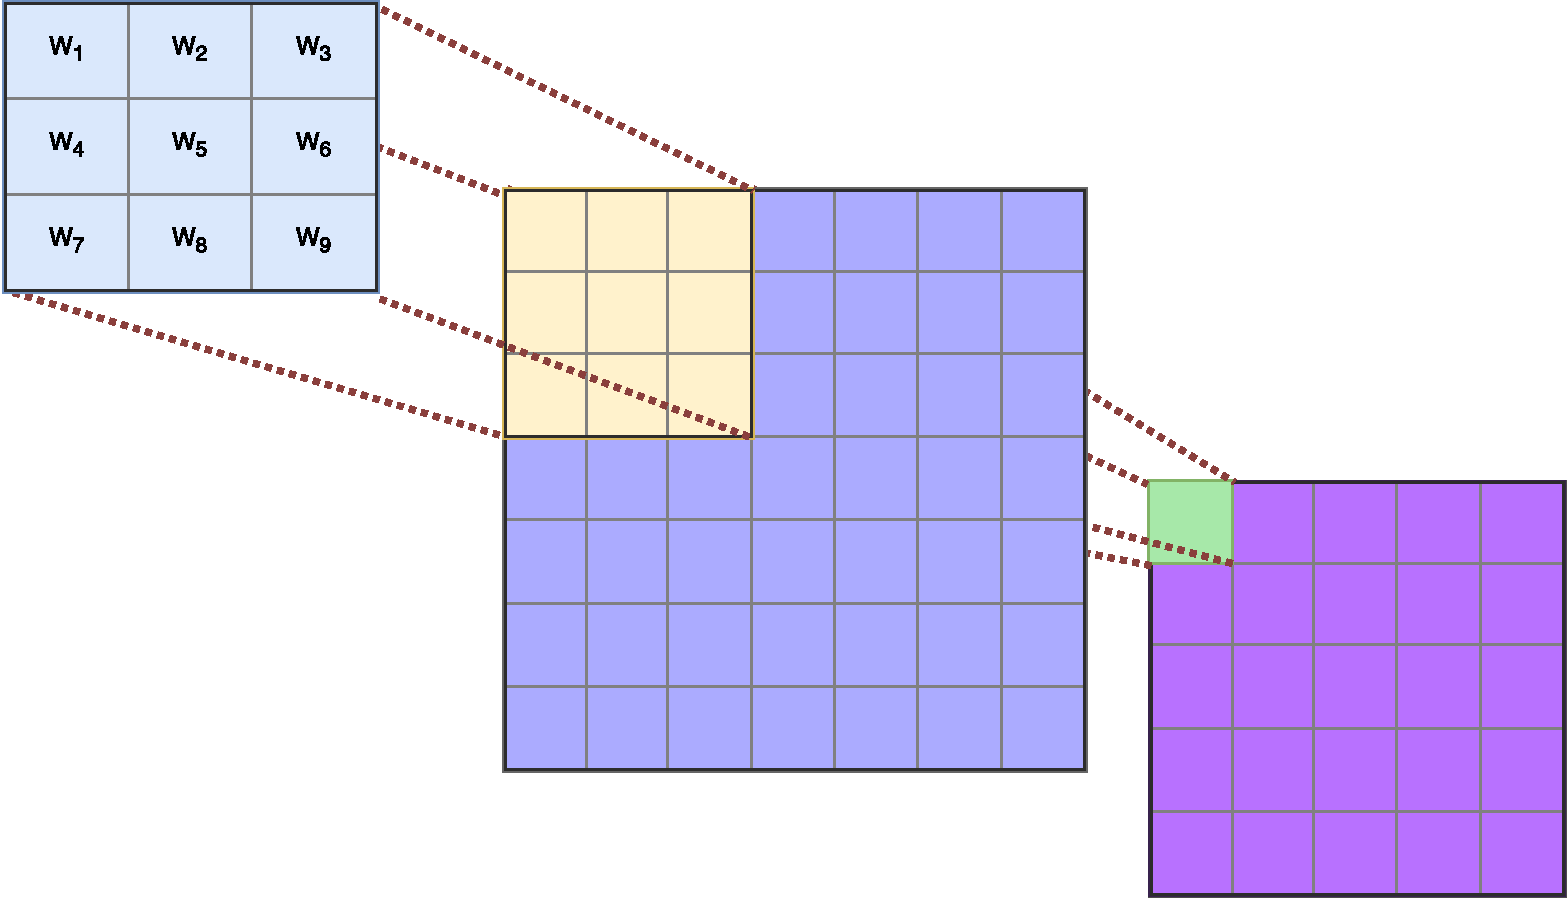
\includegraphics[width=\linewidth]{Chapters/2.Background/figures/convolution.pdf}
    \caption[Illustration of convolutional operation.]{Illustration of convolutional operation. The teal matrix contain convolutional parameters. These are element-wise multiplied by the overlapping (yellow) pixels in the image (blue) and added together. The resulting value is placed in the corresponding location in the output feature map (purple). The convolutional operation is completed by sliding or \textit{striding} the yellow window across the original image.}
    \label{fig:conv}
\end{figure}
To remedy this problem, image classification usually contain convolutional layers which are invariant to scale, rotation or translation. In a convolutional layer, a \textit{kernel} of trainable weights are convolved with the input image. This results in what is called a feature map, where the image size is reduced by some number of pixels\footnote{In some cases we would want to keep the image dimensions, in which case the input image can be padded to keep its original form.} depending on the size of the kernel, but the depth of the image (number of channels) is increased, the intent being each feature map contains more abstract information than the previous one. 

In a convolutional operation, a kernel is slid across an image, and for every overlap between the kernel and a image section, the kernel weights are multiplied with its corresponding pixel and summed (see \ref{fig:conv}). As with fully connected layers, the operations performed in each step is multiplication and summation, but here, each pixel in the output feature map contains some spatial information.
This spatial area covered by each feature can be controlled by the kernel size and how much the kernel is moved (called stride) between each kernel multiplication.
Networks consisting of multiple layers of convolution is called convolutional Neural Networks (CNNs)\footnote{These is the types of modules used in implementing the quinary MNIST classification in \ref{exp1}, and the whole of \ref{exp2}}.

\begin{figure}[ht] 
    \centering
    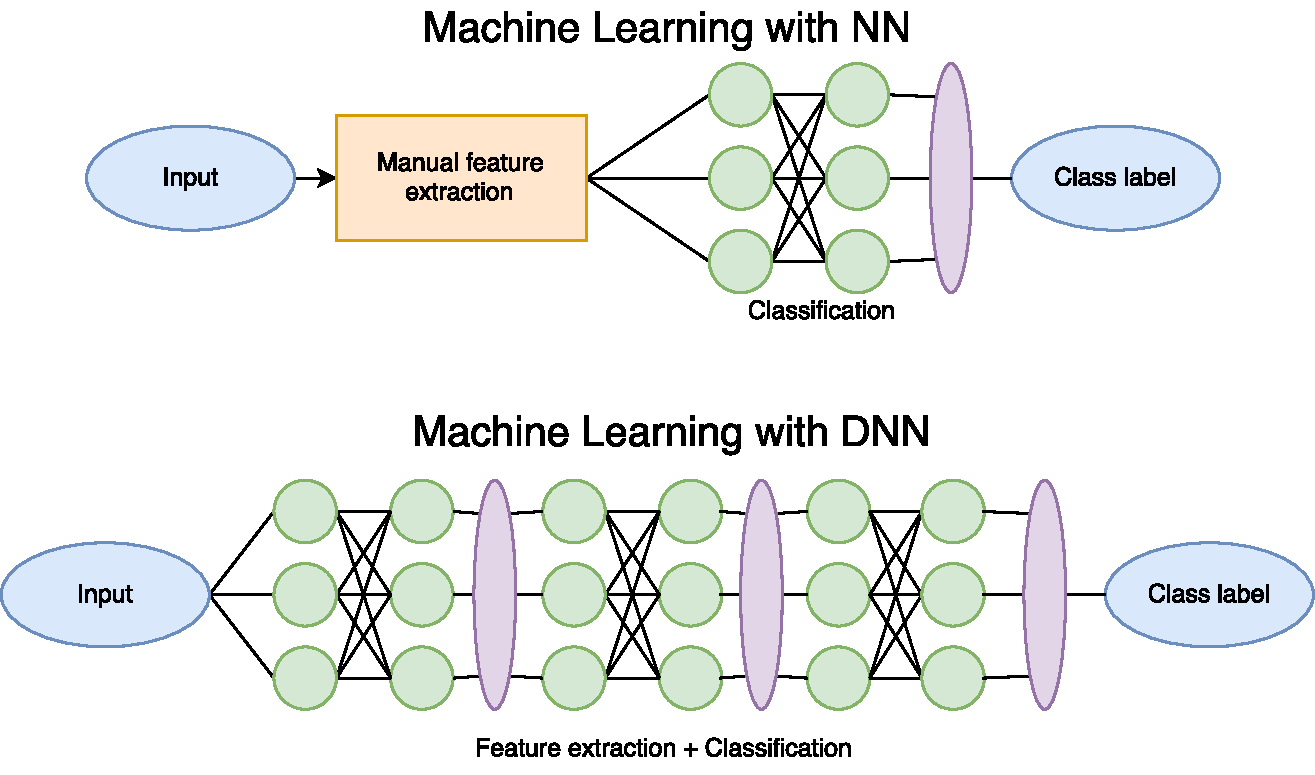
\includegraphics[width=0.8\linewidth]{Chapters/2.Background/figures/NNvsDNN.pdf}
    \caption[NN vs DNN]{Figure visualizes the difference between traditional Neural Networks and Deep Neural Networks. Artificial neurons (\textit{green}) are fully connected in both cases, and an activation layer (\textit{purple}) is set after every two layers. Where classical NN depends on being provided with high order features, the DNN performs its own feature extraction in its first layers.}
    \label{fig:NNvsDNN}
\end{figure}

\section{Deep Learning}
Usually when talking about CNNs, the line is crossed into what is described as Deep Learning. In each layer of convolution, the spatial size is reduced while the number of channels is increased. This means the information worked on for each step gradually shifts from a spatially encoded image of sorts to a encoding in feature space. This makes a full CNN capable of turning raw image input into a higher order feature representation which can be used in classification. This is why deep Convolutional Neural Networks can be said to be Neural Networks that performs its own feature extraction from raw data.

\begin{figure}
    \begin{subfigure}[h]{0.49\linewidth}
        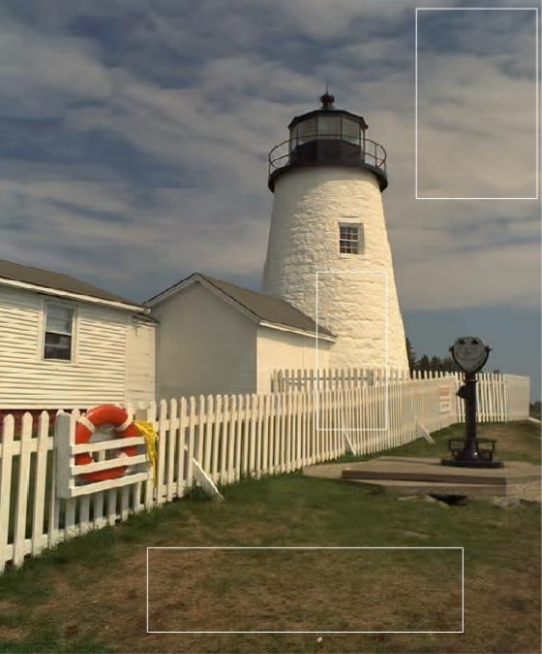
\includegraphics[width=\linewidth]{Chapters/2.Background/figures/original.png}
        \caption{Original image}
    \end{subfigure}
    \hfill
    \begin{subfigure}[h]{0.49\linewidth}
        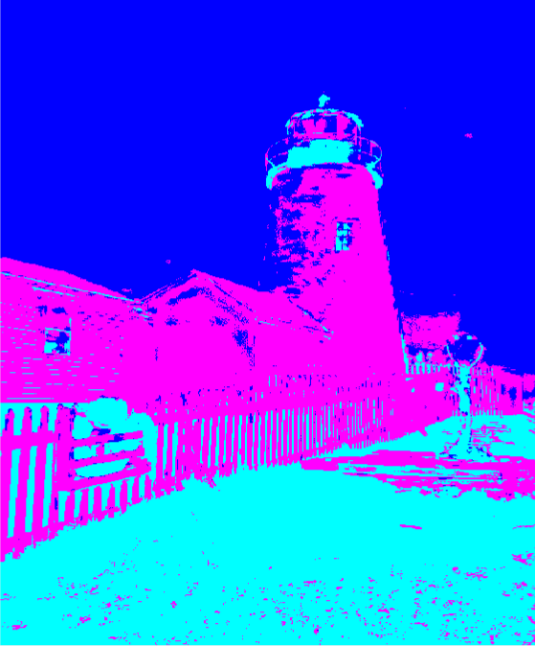
\includegraphics[width=\linewidth]{Chapters/2.Background/figures/segmentation.png}
        \caption{Segmented image}
    \end{subfigure}
    \caption[Image segmentation]{Example of image segmentation. Original image have been segmented into three classes: \textit{sky}(blue), \textit{ground}(teal) and \textit{building}(pink). The three boxes in the original image is pixels used as training data for each class.}
    \label{fig:semanticsegmentation}
\end{figure}

How \textit{deep} a DNN is made depends on the task at hand. Take for example a complex task such as \textit{semantic segmentation}. Semantic segmentation is a variation of image classification where each pixel in a input image is assigned a class label, and the whole of the image can segmented into its parts (see figure \ref{fig:semanticsegmentation}). In such a CNN, the spacial information in the original image can not be removed completely since we want to create a new image with the original dimensionality and spacial locations of objects. Such a NN would need to have enough \textit{capacity} to retain all needed knowledge to complete the task. The capacity of a NN is how much information is able to be stored in its weights, and is a measure highly correlated to the NNs number of parameters. Managing capacity needs of a NN is part of the motivation behind encouraging module reuse in experiments 1 and 2 (see chapters \ref{exp1} and \ref{exp2}).

Intuitively, the difference between NNs and Deep neural networks (DNN) is just the number of layers in the model, but functionally we can view the DNN as a collection of \textit{shallow} learning models, defined through the use of activation functions as seen in \ref{fig:NNvsDNN}. Complex Deep Learning models have been effective at such tasks as image classification\cite{imageclassification}, natural language processing\cite{deepnlp} and Reinforcement Learning\cite{deepreinforcementlearning}. The architecture and use of each of these types of DNNs are dependent on the input type and problems they are applied to as well as resource limitations.

\textbf{Edit note: Need more about DL?}

The large number of trainable parameters in deep learning increase the data resources needed. If the amount of available labeled training data is restricted, one solution is to train on a similar task for which there is a good amount of data and apply what is learned to the original task. It is shown that this reuse of knowledge as a basis for further learning yields better results that was possible with the original data set\cite{pathnet, progressiveneuralnetworks, tradaboost}. 

\subsection{Transfer Learning}
\label{background:TL}
The approach of Transfer Learning (TL) is to use generalized knowledge in one domain as a basis for future learning in another. With the goal of achieving more effective learning in the target domain or even reaching a lower convergence point for the loss, TL shares some common ground with the field of multi-task learning, where the same model is applied to multiple tasks. 

We can define transfer learning as trying to learn a target conditional probability distribution \(P(Y_{t}|X_{t})\) within a domain \(\mathcal{D}_{t}\), based on information gained from learning a source task \(\mathcal{T}_{s}\) in the source domain \(\mathcal{D}_{s}\) where \(\mathcal{D}_{s} \neq \mathcal{D}_{t}\) and \(\mathcal{T}_{s} \neq \mathcal{T}_{t}\). A domain \(\mathcal{D}\) would then, in a typical classification example, be given as \(\mathcal{D} = \{X, P(X)\}\) where \(X = x_{1},x_{2}, \dotsc ,x_{n}\) are sampled from the feature space \(\mathcal{X}\) and \(P(X)\) is a probability distribution over that space. The task \(\mathcal{T}\) in that domain would then consist of a label space \(\mathcal{Y}\) and the conditional probability distribution \(P(Y|X)\) which usually is approximated during training on a set of \(x_{i}, y_{i}\) pairs where \(x_{i} \in \mathcal{X}\) and \(y_{i} \in \mathcal{Y}\).
\newline\newline

Traditionally, transfer learning has been applied in three ways: 
\begin{enumerate}  
    \item Replacing the last layer in some trained NN. For example using the first layers of a CNN image classifier as feature extraction for some other image classification task 
    \item Fine tuning a trained NN by restarting a back propagation sequence for new data from a domain \(\mathcal{D}_{t}\)
    \item A combination of the preceding techniques where the last layers of a NN is replaced and trained from scratch, and the loss for these layers are back propagated through the rest of the already trained net.
\end{enumerate}


\begin{figure}[h] 
    \centering
    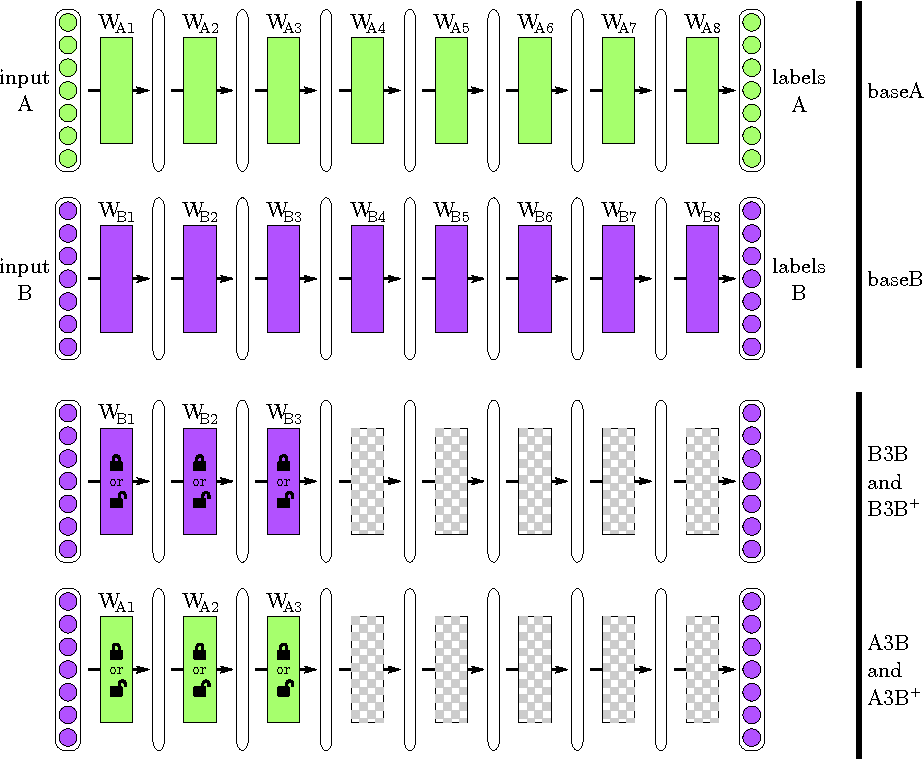
\includegraphics[width=\linewidth]{Chapters/2.Background/figures/transfer_experiment.png}
    \caption[Transfer learning experiment]{Illustration provided by Yosinski et al. in their paper\cite{yosinski2014transferable} in figure 1 to visualize their experimental process. The top two models A (green) and B (purple) are trained first on data A and data B. The labeled rectangles represents each layer in the networks, i.e. \(W_{A_{1}}\) is the weights in layer 1 in model A and the ellipsoids between each layer represents activation layers. The color of the stack of circles to the left of each model shows which partition of the data set each model is trained on(again A is green and B is purple). The bottom two rows show the first three layers from A and B being transferred to new randomly initialized models. In the paper they showed they found better accuracy in model A3B than every other model in this figure, even B3B.}
    \label{fig:transferexperiment}
\end{figure}

In a study by Yosinski et al. \cite{yosinski2014transferable}, results showed transferability in the first layers of an image classifier during an experiment proposed to measure generality and specificity in the layers as transfer performance. The study divided the data set\footnote{The study used the ImageNet dataset of 2012 which contained 1,281,167 labeled training images and 50,000 test images, each labeled with one of 1000 classes.} randomly in two subsets (A and B), and trained two identical models on each of the subsets. Replacing the first n layers in two randomly initialized other models with the first \(n\) layers from the trained models (one from A, and one from B), they did an additional training step (fine-tuning by allowing back propagation through the copied layers in some cases) on data from subset B only. This is visualized in figure \ref{fig:transferexperiment} for \(n=3\). The goal was to study the effects transferring layers from one classification case to another had on accuracy. The best results reached were achieved when training a model on subset A, transferring the first three layers to a new randomly initialized model and fine-tuning these transferred layers while training the newly formed on data from subset B. This confirmed their expectation that the earlier layers in a image classifications scenario learns to approximate Gabor-filters which are highly generalized. In section \ref{exp1:results} we see tendencies to this behaviour. 

\subsection{Multi-task Learning}
Multi-task Learning and Transfer Learning both have the same ideology of sharing some parameter state between tasks to positively influence learning. Where Transfer Learning does not concern itself with performance on a seed task, multi-task learning try to optimize parameters for multiple tasks. The most common ways of achieving this is by \textit{soft parameter sharing} and \textit{hard parameter sharing}. While both techniques have some weights unique to each task, \textit{hard parameter sharing} optimize the same parameters for all tasks. This is shown to significantly reduce overfitting\cite{hardparametersharing}. As the weights change values to optimize for a changing target, they never overly adapt to the training set. \textit{Soft parameter sharing} on the other hand have separate parameters for each task, but lateral connections between each tasks layers to minimize the distance between the parameters trained for each task.

\subsection{Curriculum Learning}
Both humans and animals learn better when examples provided is ordered and gradually increasing in difficulty. With this motivation, curriculum learning is introduced as strategy for optimizing the learning process. This technique is shown to increase generalization to data\cite{curriculumlearning} and is the motivation for task ordering in the selection pressure experiments (see \ref{exp2:datasets}).

\section{Catastrophic Forgetting}
A problem that arises in systems where parameters is trained on multiple sequential tasks is what is called \textit{catastrophic forgetting}. Not discussed by Yosinski, but set in a transfer learning scenario, this effect manifests itself as moving parameters away from an area of low error for a previously trained task. This movement could for instance be because the parameters is fine tuned for a new task. While the performance for the second task increase, performance for the first task decrease because the \textit{knowledge is forgotten} when the weights are re-adapted to the new data. This is not a problem in a scenario where the source task is considered a stepping stone to reach good performance for the target task, but might be if all tasks trained on are of the same importance.

\begin{figure}[h]
    \centering
    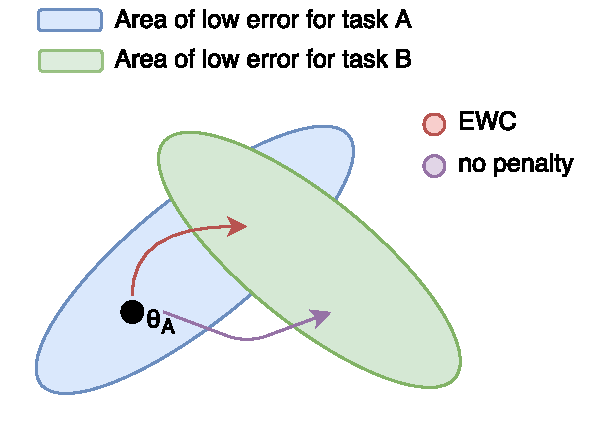
\includegraphics[width=0.7\linewidth]{Chapters/2.Background/figures/EWC.pdf}
    \caption[Elastic Weight Consolidation]{Figure from the paper on reducing catastrophic forgetting\cite{ewc}. The figure shows the parameter space \(\mathcal{P}\) and hypothetical areas of low error for two tasks A and B. The arrows indicate the direction EWC \textit{red} and normal training \textit{purple} takes the parameters.}
    \label{fig:ewc}
\end{figure}

\subsection{Elastic Weight Consolidation}
Elastic Weight Consolidation (EWC) is a novel algorithm proposed in January of 2017 by Kirkpatrick et al.\cite{ewc}. During the transfer of weights from task A to task B, over-parameterization makes it likely that a solution to problem B\footnote{A solution may be viewed as a set of parameters \(\bar{\theta}\). Training a NN consists of adjusting these parameters through the process of back propagation with the gradient descent algorithm. For multiple parameters in \(\bar{\theta}_{A}\), many configurations of those values will give the same performance for the NN.} lays close to the solution for task A in the parameter space \(\mathcal{P}\). During optimization of \(\bar{\theta}\) for task B, EWC makes sure the parameters stay within an area of low error for task A as seen in figure \ref{fig:ewc}

Using EWC, Kirkpatrick et al.\cite{ewc} was able to train the same NN on 10 different Atari games without the effects of catastrophic forgetting between training tasks. With a human-normalized score of 1 for each game, giving a total possible score\footnote{where is 0 the same as a random agent, and 10 is at least human-level performance on all games.} of 10, the EWC driven training reached a score of around 6 after 500 million training frames, while the control never reached anything higher than 1.

\subsection{Progressive Neural Networks}
Rusu et al. published a paper in September of 2016\cite{progressiveneuralnetworks} where they addressed the problem of catastrophic forgetting during transfer learning with fine-tuning. Their proposed solution, Progressive Neural Networks (PNN) were shown to be able to learn multiple tasks sequentially without overwriting the previously trained weights. This was done by horizontally scaling the DNN with a new stack of layers for each new task the structure was applied to.
\begin{figure}[h]
    \centering
    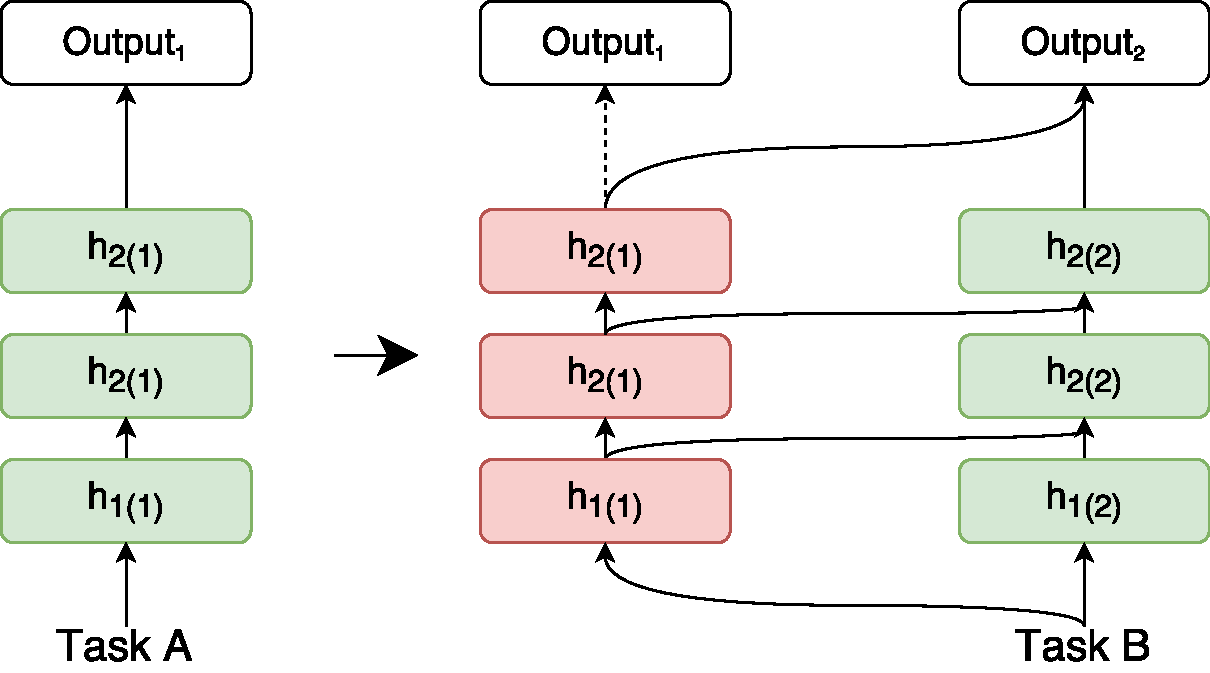
\includegraphics[width=0.8\textwidth]{Chapters/2.Background/figures/ProgressiveNeuralNet.pdf}
    \caption[Progressive Neural Network]{Example of a PNN. \textit{Left}: a three-layer NN is trained on task A. \textit{Right}: Adding another stack of three hidden layers that are being trained on task B. The weights in the first stack trained on A is now locked to the back propagation from task B, but its weights may be used is shown by arrows between the layers. Green indicates layer is open to back propagation, red indicates it is locked. Note that injection of a layer from a older task is not possible as lateral connections are only \textit{to} the new layer. The figure is a simplification of multiple figures from the article\cite{progressiveneuralnetworks}}
    \label{fig:pnn}
\end{figure}
After training a DNN on a task A\footnote{In the paper, the PNN is focused as an application for Reinforcement tasks where the PNN were trained to provide probabilities over actions from a set of possible actions, from an input state.}, a new DNN were initialized with lateral connections (see fig. \ref{fig:pnn}) to the NN trained on task A and then trained on task B with back propagation only done through the newly initialized layers. This ensures that the new DNN can optimize freely on task B, but will be able to utilize the weights trained on task A, without catastrophic forgetting occurring in the first DNN. When a sufficient performance on task B is reached, the PNN is able to perform optimally on both tasks, given some selection of the output (i.e: if given data for a task within the domain A, the output from the weights trained on task B is not optimal). Multiple tasks can be trained using this method. For each new task, a new DNN is initialized and the other DNNs in the PNN is connected laterally to each new layer. 

We can compare the way each new task is learned to a transfer learning scenario where backpropagation is locked in the transferred layers (see figure \ref{fig:transferexperiment}). The difference being the layer outputs are calculated in parallel for the two models and multiple of these outputs may be introduced in the new model through what the paper calls \textit{adapters} (not visualized in \ref{fig:transferexperiment}). These \textit{adapters} performs dimensionality reduction as well as tunable scalars so the model can scale lateral connections as needed for the new task.

A problem with this scaling raised and addressed in the paper is that of quadratic growth of parameters for each new training task. Experiments show that there is a reduction in the new capacity actually utilized by the PNN for each new task added. This implies the growth of the PNN for each new task could decrease exponentially\footnote{Here the paper suggests pruning or online compression during learning.} without needing the new task to follow the same downward trend in complexity. 

\section{Genetic Algorithms}
\label{background:GA}
Falling in a sub-category of evolutionary algorithms, genetic algorithms (GA) are biologically inspired algorithms that generate high-quality solutions to optimization and search problems. By mimicking natural operators like \textit{crossover} and \textit{mutation}, GAs views its possible solutions as individual genomes in a population, and applies these natural operators on the population in a simplification of how evolution works. 

An important driving force of GAs is the fitness-function, which maps a genome to a fitness value that can be used to rank solutions (genotypes) by how well they perform. In a natural example of the fitness function, a strong animal of some sort able to acquire nourishment and fend of potential predators is given a higher fitness value than a similar animal not as well suited for its environment. The famous term \textit{survival of the fittest} is valid in both this example and the \textit{in silico} representation of evolution. The strongest animal has a higher probability to survive and reproduce, and GAs are implemented to favour solutions that yield high fitness values.  
When a population is ranked by its fitness, different selection schemes can be applied to simulate the natural selection of the strongest genomes. This selection function have a direct influence on how diverse the population is in its solutions. While we intuitively would like to remove bad solutions and keep the strong, this might guide the population to only have the same strong genome, at which point we say the population have \textit{converged}. This causes the search to get stuck in a \textit{local optima}, where the space of possible solutions have not been explored as much as we possible would like to be able to say the solution we found are among the very best. In stead, the selection function varies which genomes are removed, where the more fit genotypes typically have a higher probability to survive. 

A much used way of order and discuss genetic algorithms is by the properties \textit{exploration} and \textit{exploitation}. A search with high exploration tries to keep a diverse population where many possible solution types are tried to find a area in solution space with high fitness. On the other hand, algorithms with high exploitation will usually find the locally best solution. A way of achieving this is by keeping a uniform population with only small differences in the genomes.

To keep the population size from shrinking, some recombination of the existing genomes is applied to increase the amount of solutions to achieve the \textit{crossover} from one generation to the next. This recombination algorithm is highly dependent on the search implemented, but they all combine two or more parent solutions to produce a offspring. Typically, a child is then mutated under some probability to further maintain genetic diversity. This mutation apply some small change to the genome.

\begin{figure}[h]
    \centering
    \begin{subfigure}[h]{0.25\linewidth}
        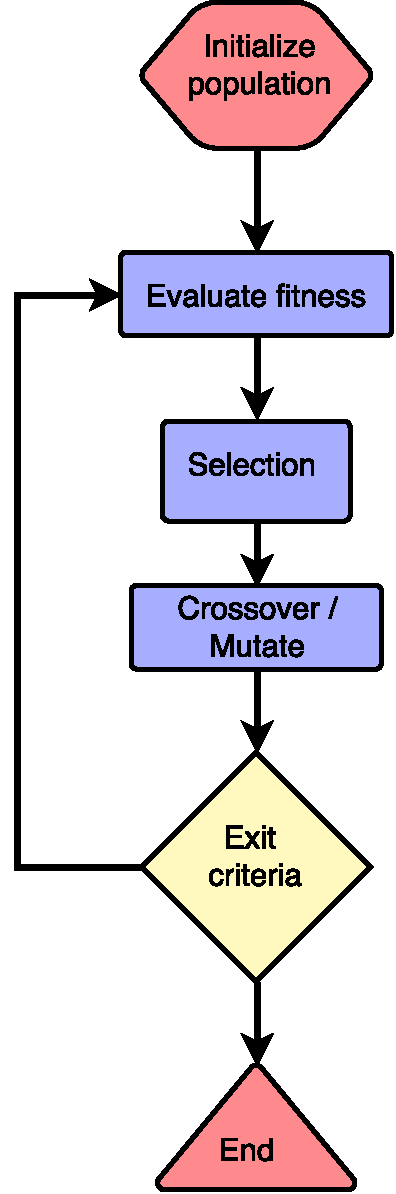
\includegraphics[width=\linewidth]{Chapters/2.Background/figures/ga_flowchart.pdf}
        %\caption{Genetic Algorithm}
    \end{subfigure}
    \hspace{0.25\textwidth}
    \begin{subfigure}[h]{0.25\linewidth}
        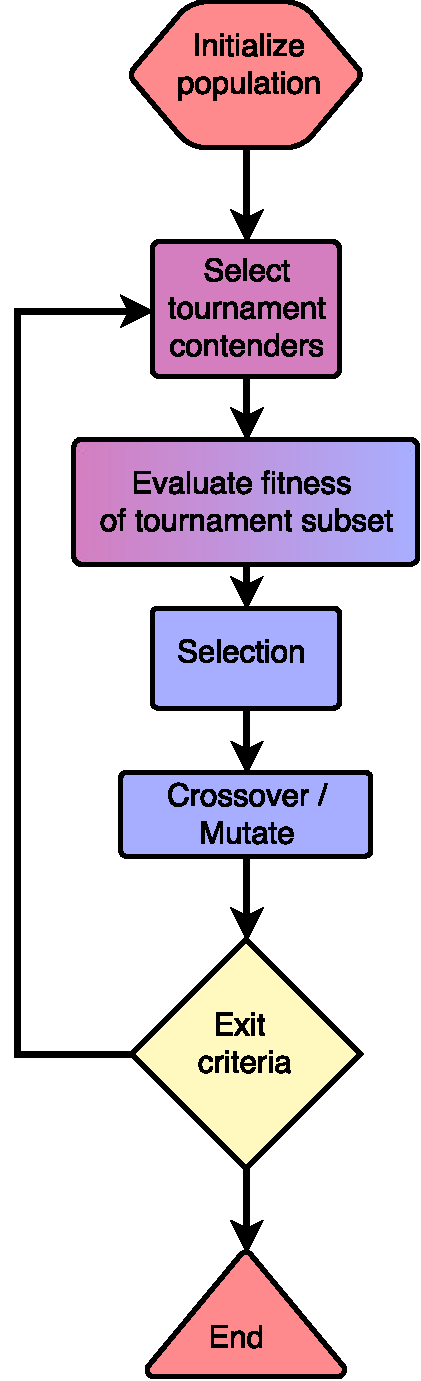
\includegraphics[width=\linewidth]{Chapters/2.Background/figures/tournamentsearch_flowchart.pdf}
        %\caption{Tournament Search}
    \end{subfigure}
    \caption[Algorithm flowcharts]{Flowcharts of the general Genetic Algorithm (left) and Tournament Search (right). The color blue indicates the operation is standard in a GA, while purple is special to a tournament search}
    \label{fig:algorithmflowcharts}
\end{figure}

\subsection{Tournament search}
One implementation of a genetic algorithm is the Tournament Search or Tournament selection. True to the name, every generation a subset of the population is selected for a tournament. The genotypes are evaluated with a fitness function and some selection scheme chooses genomes to be reinserted back into the population. The selection probability is given as 
\begin{equation}
    \label{eq:tournamentsearch}
    P_{i} = p(1-p)^{i-1}
\end{equation}
where i is the fitness-ranking achieved during the tournament (1 being first place and so on) and p the probability of choosing the winner to survive.  

In the search implementation used in the experiments in this thesis (see \ref{exp1:implementation} and \ref{exp2:implementation}), a version of the tournament search is used. For every generation, a selection of the total population given by the tournament size, is selected and evaluated. The winner then replaces each of the other contestants, making this implementation what is called a \textit{Deterministic Tournament Selection}, e.g: \(p=1\). Before the winner and its duplicate(s) is inserted back into the population, each copy of the winner is mutated under some probability to keep the diversity. 

A benefit of the tournament search, except for its efficiency in implementing and ability to work in parallel architectures, is that the \textit{selection pressure} of the search can easily be adjusted(see \ref{exp2:algorithms}). By increasing the tournament size, the winner of the tournament influence the future generations more.

\subsection{Population Diversity}
\label{background:diversity}
Mentioned here because of its importance in the experiment in chapter \ref{exp2}, population diversity is a metric assigned to a population that describes its internal difference between genomes. This value translates to how efficiently a search explores the solution space as the more similar genomes in a population are, the narrower search space is looked into. The goal of this metric is to provide a scalar value corresponding to the spread of genomes in genotypic space. 

Take for instance two binary genomes a and b as a population.
\begin{equation*}
    \begin{split}
        a = [0, 1, 1, 0, 0, 1, 1]\\
        b = [0, 0, 0, 1, 0, 1, 0]\\
        F_{\textit{Diversity}}(a, b)=x_{1}
    \end{split}
\end{equation*}
The diversity function \(F_{\textit{Diversity}}(a, b)\) gives a scalar diversity value \(x_{1}\). If we change the genome \(b\) to something more like \(a\), the new diversity \(x_{2}\) is smaller than \(x_{1}\) as the total diversity in the population has been reduced. 

\subsubsection{Pair-wise Hamming Distance}
One of the most commonly used measures of distance in genotypic space\cite{populationDiversity} is the pair-wise Hamming distance given by the equation 
\begin{equation}
    \label{eq:Hamming}
    H=\sum_{j=1}^{j=P-1}\sum_{{j}'=j+1}^{{j}'=P}\sum_{i=1}^{i=L}\left |y_{ij}-y_{i{j}'}\right |
\end{equation}
where P is the population size, L is the length of genome and \(y_{ji}\) is the i-th genome of genome j. In experiment in chapter \ref{exp2} a reduced form of this formula is used to calculate diversity. See appendix \ref{appendix:Hammingreduction} for reduction proof. While Hamming-distance provides a good metric for diversity, some cases can cause Hamming-distance to misrepresent a change in diversity. 

Take f.eks the populations 
\begin{equation*}
    \begin{split}
        [0, 0, 1, 1]\\
        [1, 1, 0, 0]\\
        [1, 0, 0, 1]\\
    \end{split}
\end{equation*}
which have 3 separate genotypes and a Hamming distance of 8. Reducing the diversity in this population by setting the third genome to be equal to the second changes the population to 
\begin{equation*}
    \begin{split}
        [0, 0, 1, 1]\\
        [1, 1, 0, 0]\\
        [1, 1, 0, 0]\\
    \end{split}
\end{equation*}
changes the diversity in a obvious way, but the Hamming distance is still 8 making the Hamming metric misrepresenting the diversity when duplicates of genomes appear in a population. 

\subsubsection{Frequency Diversity}
While pair-wise Hamming distance falls short for some cases where genomes are duplicated, counting the amount of unique genomes (which would be three for the first population and two for the second) manages those cases very well. As a diversity metric by itself however, it is quite poor as there is no nuance to what is considered a unique genome. For a population of two identical genomes, changing one gene in one of the genomes would increase the diversity by the same amount as changing all genes. 

In the experiments in chapter \ref{exp2} both frequency diversity and Hamming distance is used to create a full picture of how the diversity changes during a search.

\section{PathNet}
\label{background:pn}
In 2017, DeepMind took the modular approach\footnote{Modular with respect to the traditional approaches of transfer from monolithic models} to deep transfer learning for multi-task systems one step further with their newly developed Super Neural Network structure\footnote{Super Neural Network are a meta-network where each node in the network is itself a Neural Network.}; \textit{PathNet}\cite{pathnet}. Where Progressive Neural Networks transfer knowledge between domains by adding a new uninitialized DNN for each task, the size of PathNet is not dynamic in the number of parameters. At training start, the net consists of randomly initialized weights in multiple DNNs, where each DNN is considered a module (or node) in a the larger PathNet structure. 

Using a combination of evolutionary and machine learning techniques, PathNet shares the PNNs traits of being able to optimize for multiple training tasks without catastrophic forgetting and transfer knowledge between tasks by reusing weights locked to backpropagation.  
\begin{figure}[h]
    \centering
    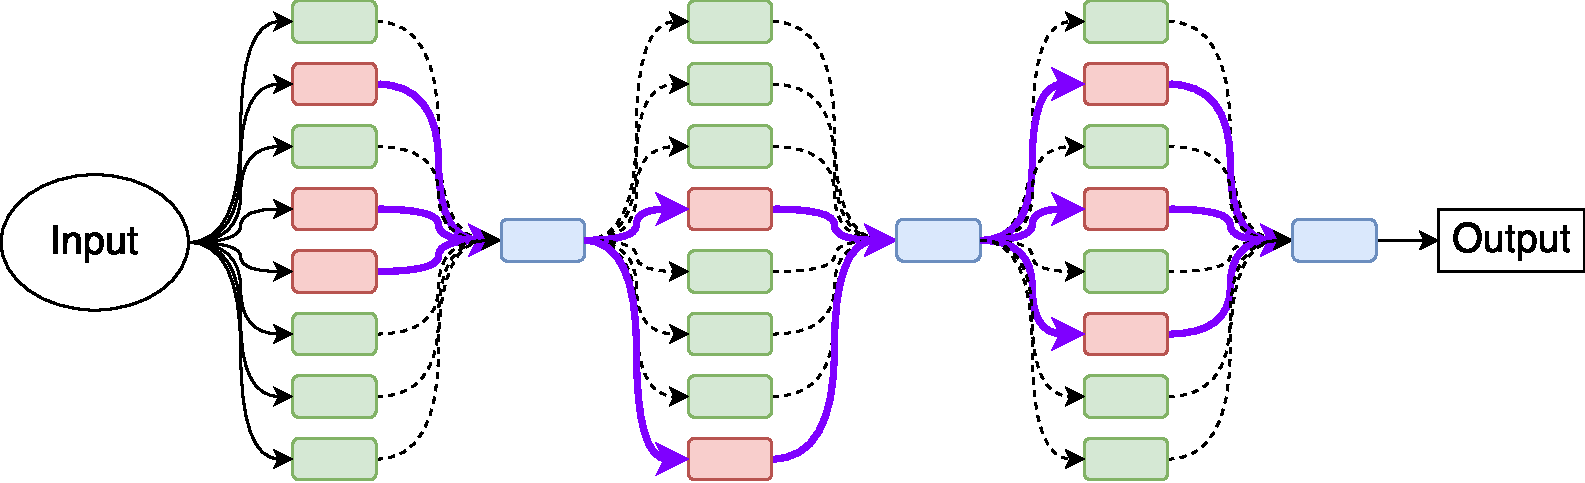
\includegraphics[width=0.8\textwidth]{Chapters/2.Background/figures/PathNet.pdf}
    \caption[PathNet structure]{Figure shows a PathNet implementation with 3 layers of 8 modules (NNs) in each layer. The \textit{red} color indicates the weights of this NN is locked to back propagation, while \textit{green} indicates it is open. \textit{Blue} cells are reduced-sum modules which summarizes the features between each layer. The purple connections show a path through the network. One path may use multiple modules from each layer, and may contain both locked and open modules.}
    \label{fig:pathnet}
\end{figure}

\subsection{Structure}
The PathNet consists of layers of modules, where each layer as a set number of modules as seen in figure \ref{fig:pathnet}. Each module is in itself a neural network of some sort, where the type of NN is adapted to the relevant task. Between each layer the output from each active module is passed through a reduced-sum operator that adds together each output element-wise to keep the dimensionality of the output from scaling by the number of active modules. 

Each task applied to PathNet is designated its own unique end-layer added to every path created for that task, meaning all paths in a search has the same final layer specific to that task. This layer defines the output and activation function to fit the problem at hand, be it classification, regression or something else.  

A \textit{path} is the name given a subset of the modules in a PathNet structure, where the path may contain between 1 and \(\omega\) modules from each layer, where \(\omega\) is adjusted to control the amount of capacity (number of weights) allocated to a path (solution). Each module in this path is locked after training is completed. This locking of the modules is to prevent the weights in the modules from changing if they are reused by subsequent tasks, and this preventative measure is what ensue catastrophic forgetting does not occur in this structure. After a optimal paths modules are locked, the rest of the modules that are not used in any path and does not contain optimized weights for a task is reinitialized. Fernando et al. claims\cite{pathnet} that this re-initialization is because they were not able to reach results that outperformed fine-tuning without it.

\subsection{Search}\label{background:pathnet.search}
For every new task introduced to the PathNet, a tournament search algorithm is initialized to find a optimal path through the network. A population of pathways (e.g: subsets of modules) are randomly initialized, and applied a tournament search with a tournament size of 2 and probability \(p=1\) of selecting the winner (as per equation \ref{eq:tournamentsearch}), making this tournament implementation deterministic. Every fitness evaluation of the tournament contenders is done by training them each a set amount and using the negative loss as a fitness value. One \textit{training unit} is quite small at 50 batches of 16 examples each. This means that evaluating the fitness of a path changes the performance of that path, unless all modules in that path is locked to backpropagation.

When a winner is selected, the genome of the winner is duplicated to replace the looser and then mutated by each module in the path having a probability \(\frac{1}{L\omega}\) of being replaced with a neighbouring module\footnote{A module with index \(i\) is replaced with a module of index between \(i-2\) and \(i+2\)}, where L is the number of layers, and \(\omega\) is as mentioned the max number of active modules in each layer. The rather large mutation rate ensures that the average path, even if it contains the maximum number of modules, would have a genome change to separate it from the winner. Over multiple generations, however, the population converges to a lower diversity state where more and more paths contain similar modules. The search is terminated under some criteria, either a reached threshold fitness or a generation limit. 
\textbf{Edit note: More about pathnet needed? implementation details? Discussion about the experiments done in \cite{pathnet}?}

\newpage

\section{Statistical methods}
\subsection{Monte-Carlo probability estimation}
\label{mc-estimate}
Given the nature of the systems used in this thesis, analytically calculating the probability of certain outcomes\footnote{In experiments \ref{exp1} and \ref{exp2}, the amount of module reuse for a random path selection is used as a comparison to experimental outcomes.} is quite hard. In such cases the probability of certain outcomes can be estimated with a Monte-Carlo approach. This is done by simulating some scenario governed by some stochastic properties for \(n\) number of trials and measuring some \(N\) number of outcomes. The probability \(p\) of these outcomes occurring can be estimated as 
\begin{equation*}
    \hat{p}=\frac{N}{n}
\end{equation*}
Since the error here is non-biased random with a mean error of zero, the standard deviation can be given as the square root of the mean squared error 
\begin{equation*}
    \sigma=\sqrt{E[(\hat{p}-p)^{2}]} =\sqrt{\frac{p(1-p)}{n}}
\end{equation*}


Selecting a sufficiently large \(n\) can be a problem with the Monte-Carlo approach since \(p\) is unknown. Still, we can for a fixed \(n\) select a maximum standard deviation we want and calculate the size of \(p\) at which point we lose accuracy. 

For a maximum ratio between the standard deviation \(\sigma\) and \(p\) of \(R\)\footnote{I.e: \(R=0.01\) means the probability of the measured outcome is 100 times larger than the standard deviation} and \(n\) being the number of trials, we can calculate maximum of \(p\) as
\begin{equation*}
    \frac{\sqrt{E[(\hat{p}-p)^{2}]}}{p} < R
\end{equation*}
\begin{equation*}
    \frac{1}{p}\sqrt{\frac{p(1-p)}{n}} < R
\end{equation*}
\begin{equation*}
    \frac{1-p}{np} < R^{2}
\end{equation*}
\begin{equation*}
    \frac{1}{p}< nR^{2}+1
\end{equation*}
\begin{equation}
    \frac{1}{nR^{2}+1}<p
    \label{eq:montecarloP}
\end{equation}
This means if we perform a Monte-Carlo simulation of \(10^{6}\) trials and we want the standard deviation to be at most \(0.01p\) the we lose certainty if the probability is smaller than \(\frac{1}{101}\).

\subsection{Comparing results}
When comparing observations during experimentation, hypothesis-testing is a way of providing gravitas to observational differences. A method is used to test a statement about the data (called a null-hypothesis or \(H_{0}\)) by providing a p-value. This p-value is compared to a predetermined significance level (usually 0.05) and provides a metric that describes the likelihood of the null-hypothesis being valid\footnote{A low p-value corresponds to a low likelihood.}. The assumption being we can claim an assumption to be true if the counter-claim is unlikely.  

\subsubsection{Mann–Whitney–Wilcoxon test}
\label{background:mannwhitney}
When calculating a P-value, the effectiveness of the method used depends highly on the observations tested. In this thesis we can not assume normality in the data, nor equal variance. Therefore a non-parametric method for comparison is used: Mann-Whitney-Wilcoxon (MWW) testing. This test provides a U-value used to reject or accept the null-hypothesis that two groups of observations have the same distribution. 

The assumptions laying behind the use of MWW are 
\begin{itemize}
    \item Rank-able continuous or ordinal data.
    \item Independent groups.
    \item Independencies in observations between groups.
    \item Whether the two distributions have the same or different shape is known. 
\end{itemize}
These assumptions are determined to be met in the case of these experiments. 

A the cases MWW is applied here contains small groups of observations, the direct explanation of how a U-value is calculated is the quickest. 

For two groups of observations, each observation is ranked by its value\footnote{In the case of the experiments in chapter \ref{exp2} and \ref{exp3} the observations are classification validation accuracies and each trials result is naturally ranked by this accuracy-value.}. The U-value for the group \(i\) is given as 
\begin{equation*}
    U_{i} = R_{i}-\frac{n_{i}(n_{i}+1)}{2}
\end{equation*}
where \(R_{i}\) is the sum of ranks in group \(i\) and \(n_{i}\) is the number of observations in that group. 
Calculating a \(U_{i}\) for each group tested provides two U-values where the smallest one is compared to a critical U value where the null-hypothesis is rejected if 
\begin{equation*}
    min(U_{1}, U_{2}) \leq U_{\text{Critical}}
\end{equation*}

\subsubsection{Bonferroni correction}
As the MWW rank-sum test is not multivariate, multiple test are performed in sections \ref{exp2} and \ref{exp3} to compare all algorithms. Because the scaling probability that some of the results are unlikely, a Bonferroni correction of the significance level is done to combat the increasing probability of encountering unlikely results. 

A desired significance level \(\alpha\) is scaled by the inverse of the number of tested hypotheses \(m\). 
\begin{equation*}
    \alpha=\frac{\alpha_{\text{Desired}}}{m}
\end{equation*}




\iffalse
    x   What is the required background knowledge? 
    x   Where can I find it? 
    x   What is the relevant prior work? 
    x   Where can I find it? 
    Why should it be done differently? 
    x   Has anyone attempted your approach previously? 
    x   Where is that work reported? 
    \Section{Nifty Gadgets my way}
    What is the outline of your way? 
    Have you published it before?  
\fi